\documentclass[journal=jacsnano,manuscript=article]{achemso}
\usepackage{chemformula} % Formula subscripts using \ch{}
\usepackage[T1]{fontenc} % Use modern font encodings
\newcommand*\mycommand[1]{\texttt{\emph{#1}}}
%\DeclareCaptionFormat{myformat}{#1(Online color)#2#3}
%\newenvironment{myfigure}%
%{\captionsetup{format=myformat}%,labelsep=period}
%\figure
%}%
%{\endfigure}%
%\usepackage{lineno}
\linenumbers
\DeclareCaptionFormat{cancaption}{#1#2#3\par}
\DeclareCaptionLabelFormat{cancaptionlabel}{#1 S#2}
%%%%%%%%%%%%%%%%%%%%%%%%%%%%%%%%%%%%%%%%%%

\author{Ganesh Ghimire} 
\email{gangh@dtu.dk}
\affiliation{Department of Electrical and Photonics Engineering, Technical University of Denmark, Denmark}

\author{Rajesh Kumar Ulaganathan} 
\affiliation{1 Centre for Nanotechnology, Indian Institute of Technology Roorkee, 247667, India}

\author{Oleksii Ilchenko}
\affiliation{Department of Health Technology Nanoprobes, Technical University of Denmark, Denmark}
\alsoaffiliation{Lightnovo, Blokken 15, 1, tv. 3460 Birkerod, Denmark}

\author{Arias Juan Camilo} 
\affiliation{Department of Electronics and Nanoengineering, Aalto University, Espoo, Finland}

\author{Claudia Piccinini} 
\affiliation{Department of Electrical and Photonics Engineering, Technical University of Denmark, Denmark}

\author{Yurii Pilhun}
\affiliation{Lightnovo, Blokken 15, 1, tv. 3460 Birkerod, Denmark}

\author{Eunji Lee}
\affiliation{Department of Energy Science, Sungkyunkwan University, South Korea}

\author{Krishna P. Dhakal}
\affiliation{Department of Energy Science, Sungkyunkwan University,  South Korea}

\author{Jeongyong Kim}
\affiliation{Department of Energy Science, Sungkyunkwan University,  South Korea}

\author{Battulga Munkhbat} 
\affiliation{Department of Electrical and Photonics Engineering, Technical University of Denmark, Denmark}

\author{Sun Zhipei} 
\affiliation{Department of Electronics and Nanoengineering, Aalto University, Espoo, Finland }
\author{Stela Canulescu}
\affiliation{Department of Electrical and Photonics Engineering, Technical University of Denmark, Denmark}
\email{stec@dtu.dk}

\title{Polarization sensitive photodetection and anisotropic optical response in \ch{MoS2} nanoribbons }

\title{Supplementary Information: Polarization-Sensitive Photodetection and Anisotropic Optical Response in \ch{MoS2} nanoribbons }
\begin{document}
\captionsetup[figure]{format=cancaption,labelformat=cancaptionlabel}
\newpage
\section*{Supplementary Note 1: Measurement schematic for sample-rotation configuration}
\begin{figure}
    \centering
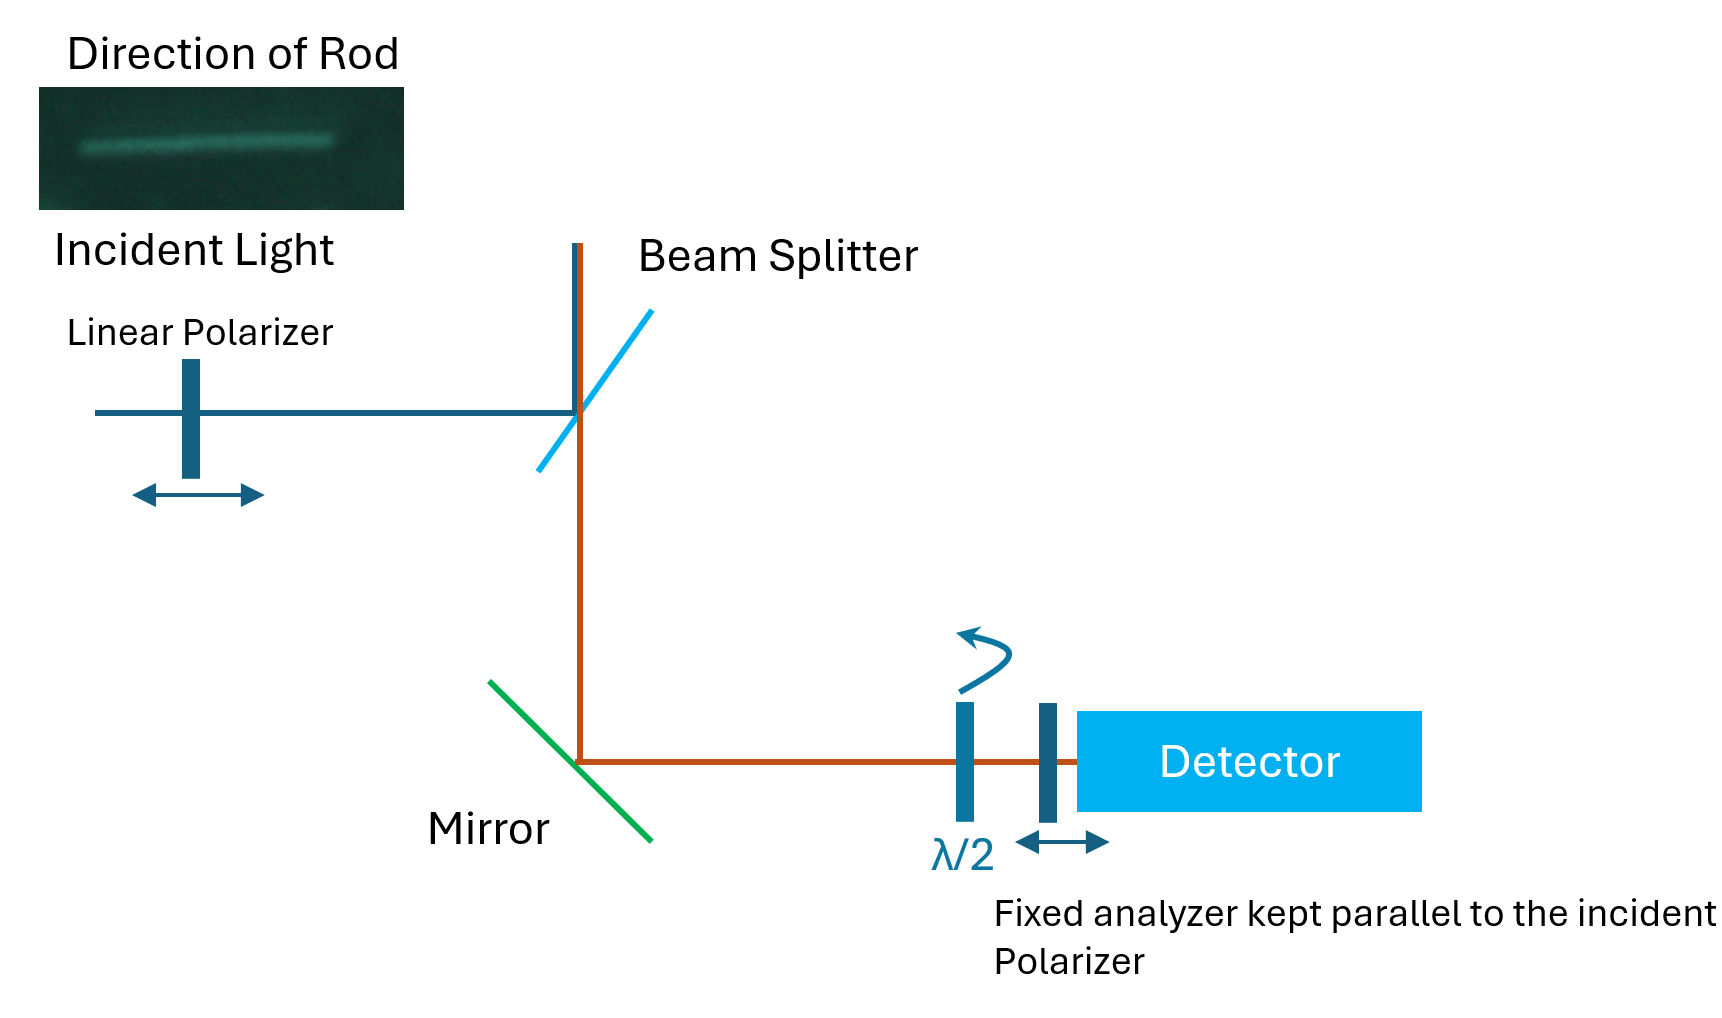
\includegraphics[width=0.9\linewidth]{Figures SI/Figure S1_setup Raman Pol.png}
\caption{\textbf{Schematic of the polarization-resolved measurement setup used for sample rotation experiments.} Experimental Linearly polarized incident light is directed onto the MoS$_2$ nanoribbon through a beam splitter, with the polarization axis defined relative
to the ribbon orientation. The reflected beam is routed to the detector after passing
through a rotatable $\lambda/2$ wave plate and a fixed analyzer kept parallel to the
incident polarizer. During the measurement, the sample is rotated while the detection
polarization remains fixed, enabling the extraction of angle-dependent optical
responses.}
    \label{fig:schematic sample rotation}
\end{figure}

Figure~S\ref{fig:schematic sample rotation} illustrates the optical configuration used to measure the polarization-dependent
response of the MoS$_2$ nanoribbons under sample rotation. A linearly polarized beam is first
generated using a linear polarizer, whose transmission axis defines the incident
polarization direction. The sample  is mounted on a 
rotation, and we obtained a series of Raman spectra while rotating the sample between a fixed polarizer and analyzer, with the rotation performed about the horizontal $x$-axis of the Raman microscope sample stage. In this configuration, the reported angles correspond directly to the rotation angle of the sample relative to the horizontal $x$-axis on the
 stage such that its long axis rotates with respect to the fixed incident polarization,
while the optical path of the excitation beam remains unchanged.


The incident beam is directed onto the sample through a beam splitter, and the reflected
signal is routed toward the detection path via a mirror. A half-wave plate ($\lambda/2$) is placed
before the detector to maintain a constant detection polarization condition; throughout the
measurement, the analyzer is kept parallel to the incident polarizer to ensure that only the
sample-induced modulation is recorded. In this configuration, the polarization state of the illumination is fixed, and the sample
itself is physically rotated from $0^\circ$ to $360^\circ$. This approach allows direct probing of
intrinsic optical anisotropy in the nanoribbons, as any change in optical intensity arises solely
from the orientation-dependent light–matter interaction rather than variation in incident
polarization conditions.

\section{Supplementary Note 2: Polarization-Resolved Raman Response of Rotated \ch{MoS2} Nanoribbons}
To further confirm the anisotropic vibrational properties of quasi–1D \ch{MoS2} nanoribbons, we performed angle-resolved Raman spectroscopy by physically rotating the sample from $0^{\circ}$ to $360^{\circ}$ while keeping both the incident and scattered light polarizations fixed. Figure~S\ref{fig:si_Mo_ribbon-Sample rotation} a,b show representative Raman spectra collected at multiple rotation angles, where the evolution of the $E^{1}_{2g}$ (in-plane) and $A_{1g}$ (out-of-plane) modes can be clearly traced.

A pronounced angular modulation is observed for both Raman-active modes, demonstrating that the vibrational response of the nanoribbon is strongly orientation dependent. The polar plots in Figure~S\ref{fig:si_Mo_ribbon-Sample rotation} c,d show that the $A_{1g}$ mode exhibits a strong twofold symmetry with well-defined maxima and minima, indicating that out-of-plane vibrations couple differently to the optical field depending on the ribbon axis. In contrast, the in-plane $E^{1}_{2g}$ mode shows a weaker but distinct anisotropy, consistent with modification of the in-plane force constants due to lattice distortion or symmetry breaking in the reduced-dimensional geometry.

\begin{figure}
    \centering
    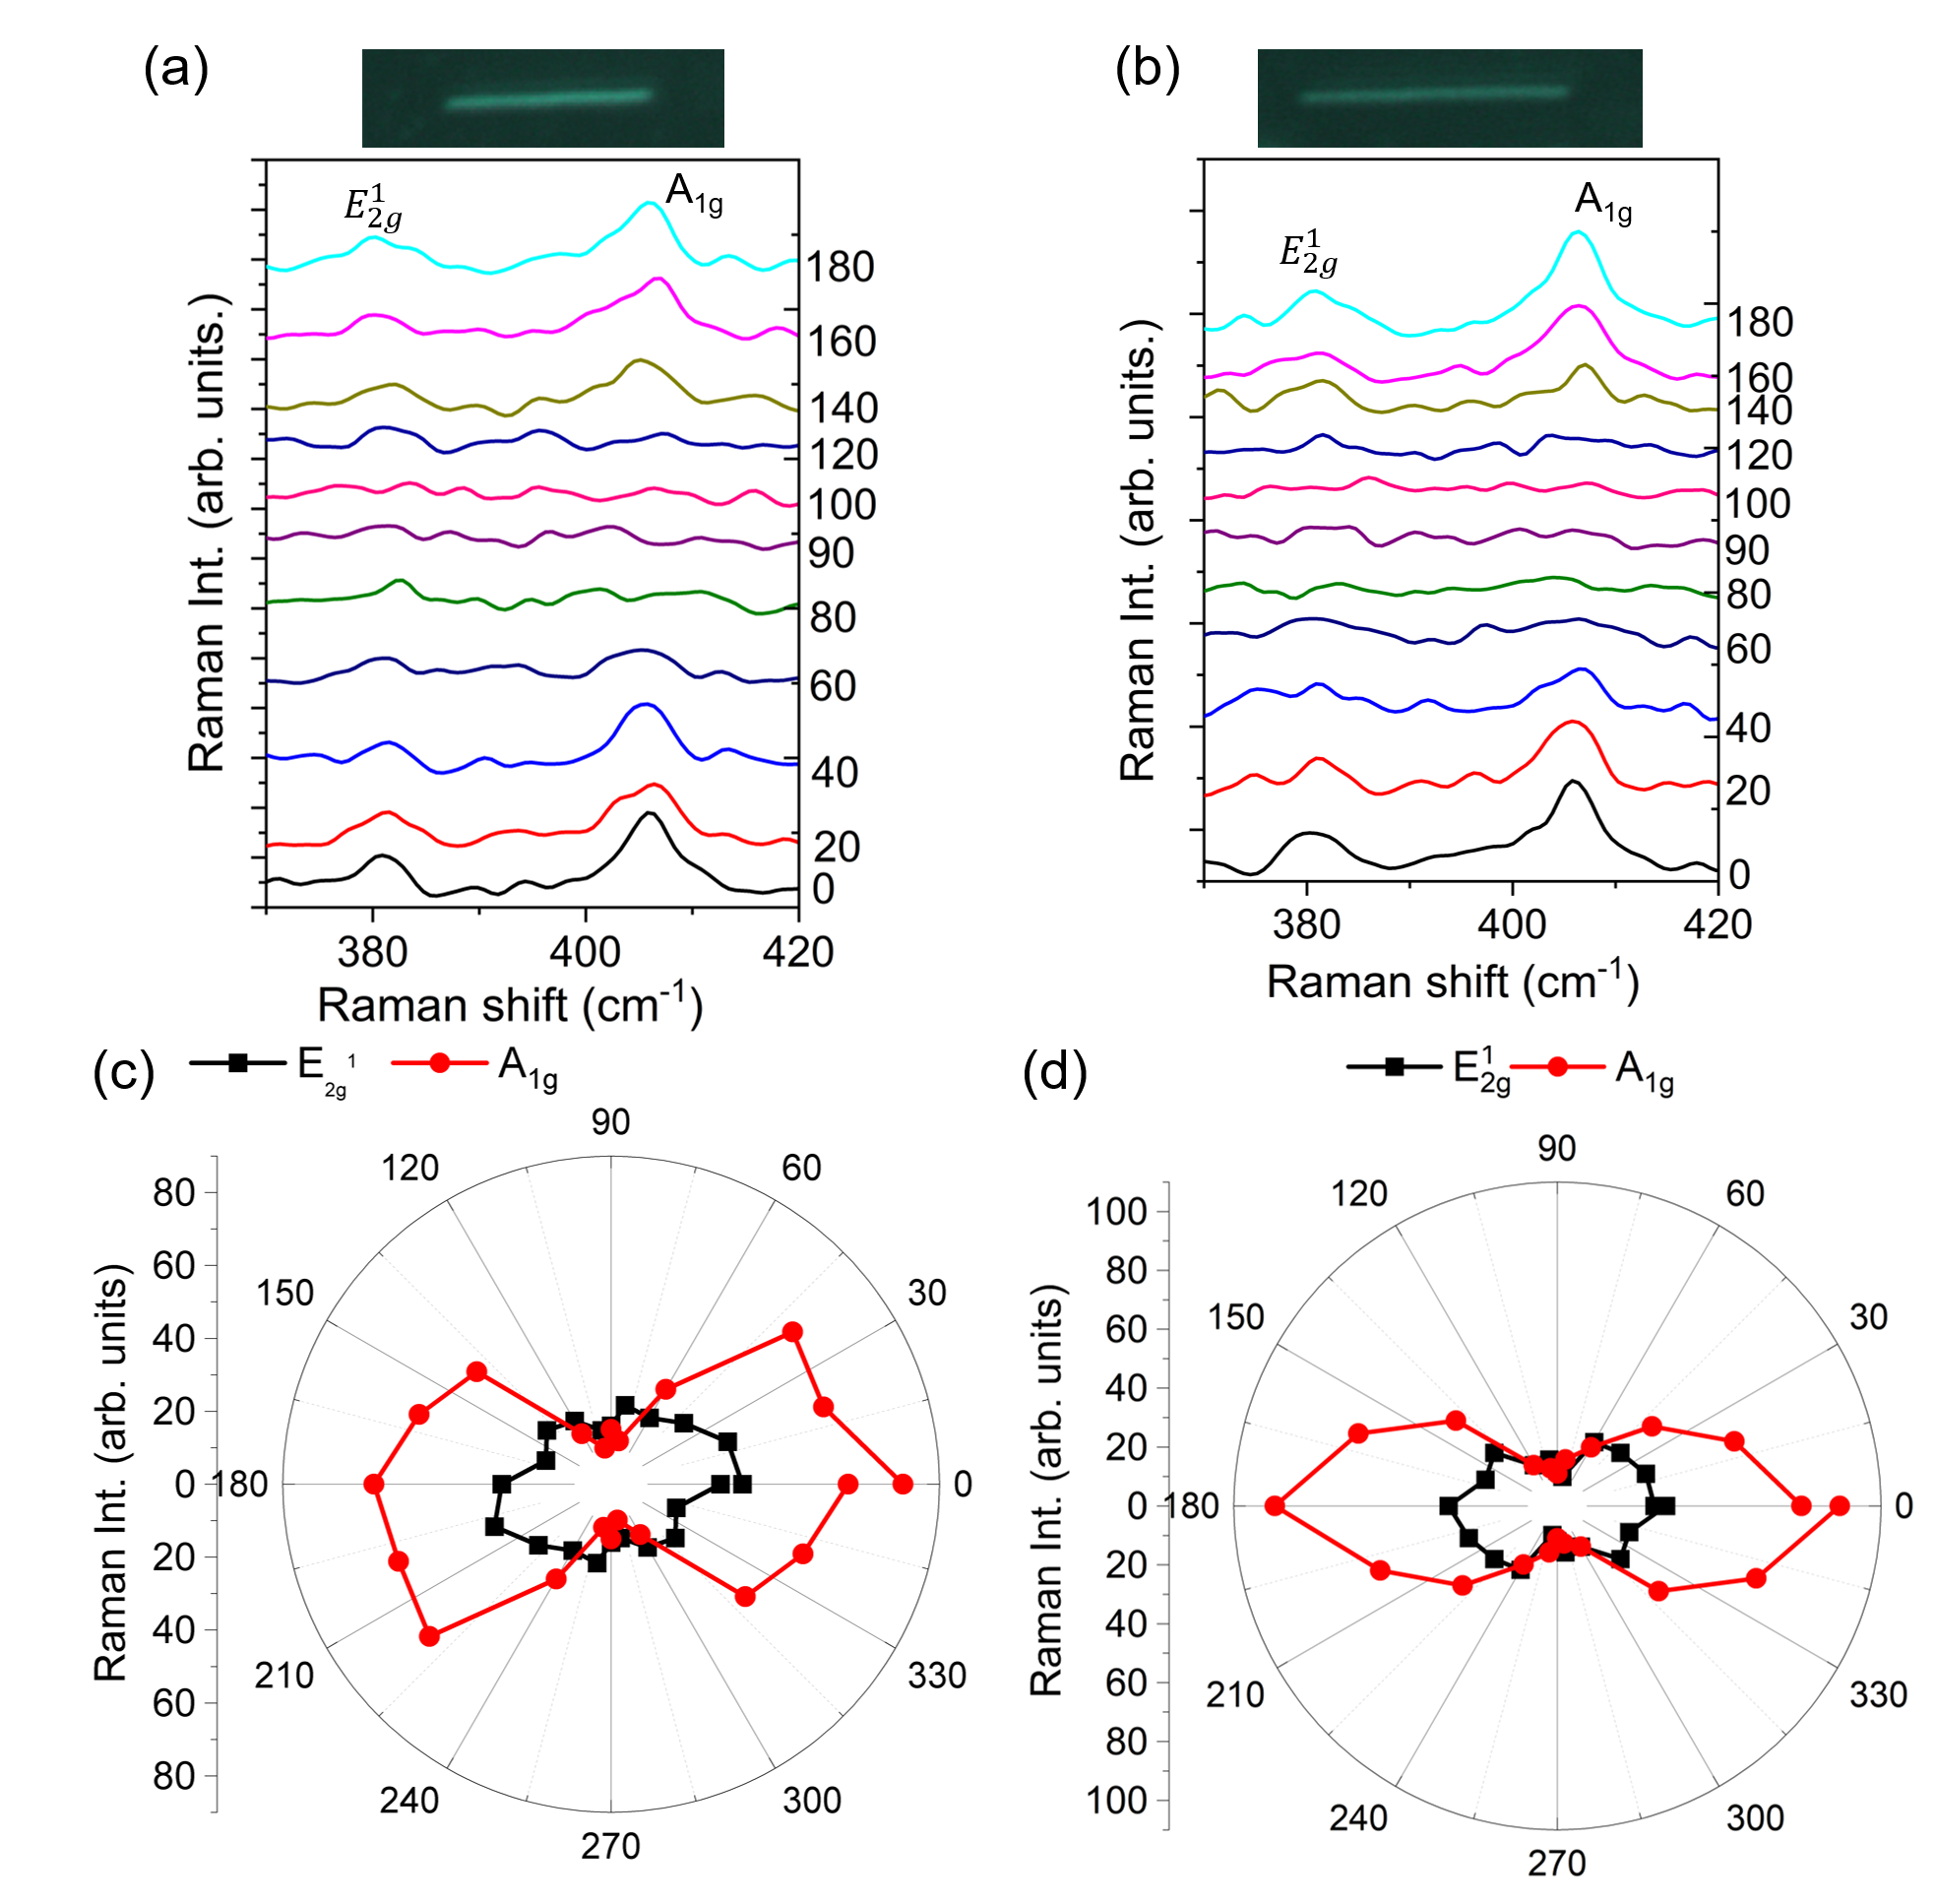
\includegraphics[width=0.9\linewidth]{Figures SI/Figure S2_polRaman rods.png}
    \caption{\textbf{Sample–rotation–dependent Raman spectroscopy of MoS\textsubscript{2} nanoribbons.}. (a,b) Raman spectra of a MoS\textsubscript{2} nanoribbon recorded at different sample rotation angles, of two different nanoribbons showing the evolution of the $E_{2g}^{1}$ and $A_{1g}$ modes. 
(c,d) Polar plots of the integrated intensities of the two Raman modes, revealing pronounced angular anisotropy arising from the quasi-1D geometry of the nanoribbon.}
    \label{fig:si_Mo_ribbon-Sample rotation}
\end{figure}
This behavior differs fundamentally from monolayer or bulk \ch{MoS2}, where the Raman tensor is isotropic under rotation due to hexagonal symmetry. The strong anisotropy observed here is therefore a direct consequence of the quasi–1D morphology of the nanoribbon, which introduces preferential bonding directions, strain gradients, and modified local dielectric screening. These effects collectively distort the Raman tensor elements, leading to angle-dependent scattering intensities. The combined evolution of the $E^{1}_{2g}$ and $A_{1g}$ modes under rotation thus provides robust experimental evidence of symmetry lowering in the nanoribbons. These results support the main-text conclusion that dimensional reduction from 2D to quasi–1D geometries produces pronounced vibrational and optical anisotropy, reinforcing the potential of \ch{MoS2} nanoribbons as polarization-sensitive building blocks for next-generation photonic and optoelectronic devices. 
\section*{Supplementary Note 3: Polarization-Dependent Raman Response of Monolayer Triangular \texorpdfstring{MoS$_2$}}

To validate the anisotropic Raman behaviour observed in quasi-1D MoS$_2$ nanoribbons, we performed identical sample-rotation Raman measurements on a monolayer triangular MoS$_2$ flake. Owing to its 2H crystal structure with sixfold in-plane symmetry, a monolayer MoS$_2$ is expected to exhibit a fundamentally different angular Raman response compared to low-symmetry nanoribbons.

Figure~S\ref{fig:si_2D_Triangular MoS2} a shows the angle-resolved Raman spectra measured while rotating the monolayer from $0^{\circ}$ to $180^{\circ}$ under fixed incident and detection polarization. Two prominent phonon modes, the in-plane $E^1_{2g}$ and the out-of-plane $A_{1g}$, are clearly resolved. Their polarization behaviour, summarized in the polar plots in Figure~S\ref{fig:si_2D_Triangular MoS2} b, reveals the characteristic selection-rule–driven anisotropy of monolayer MoS$_2$.
The $E^1_{2g}$ mode shows nearly isotropic intensity with rotation, consistent with its doubly degenerate in-plane vibrational nature and the rotational symmetry of the hexagonal lattice. In contrast, the $A_{1g}$ mode exhibits a pronounced two-lobe polar pattern, reflecting its out-of-plane displacement character and well-established dependence on the relative orientation between the incident polarization and the crystal axes. This distinct response weak angular modulation of $E^1_{2g}$ and strong modulation of $A_{1g}$ is a hallmark of monolayer 2H-MoS$_2$ and serves as an internal reference confirming the crystalline quality and symmetry of the triangular flake. The isotropic behaviour of the $E^1_{2g}$ phonon in the monolayer stands in sharp contrast to the strong Raman anisotropy observed in MoS$_2$ nanoribbons. This comparison highlights that the pronounced anisotropy in the nanoribbons originates not from the intrinsic symmetry of MoS$_2$, but from symmetry breaking induced by lateral confinement, edge structure, and quasi-1D geometry.
\begin{figure}%[htb]
    \centering
    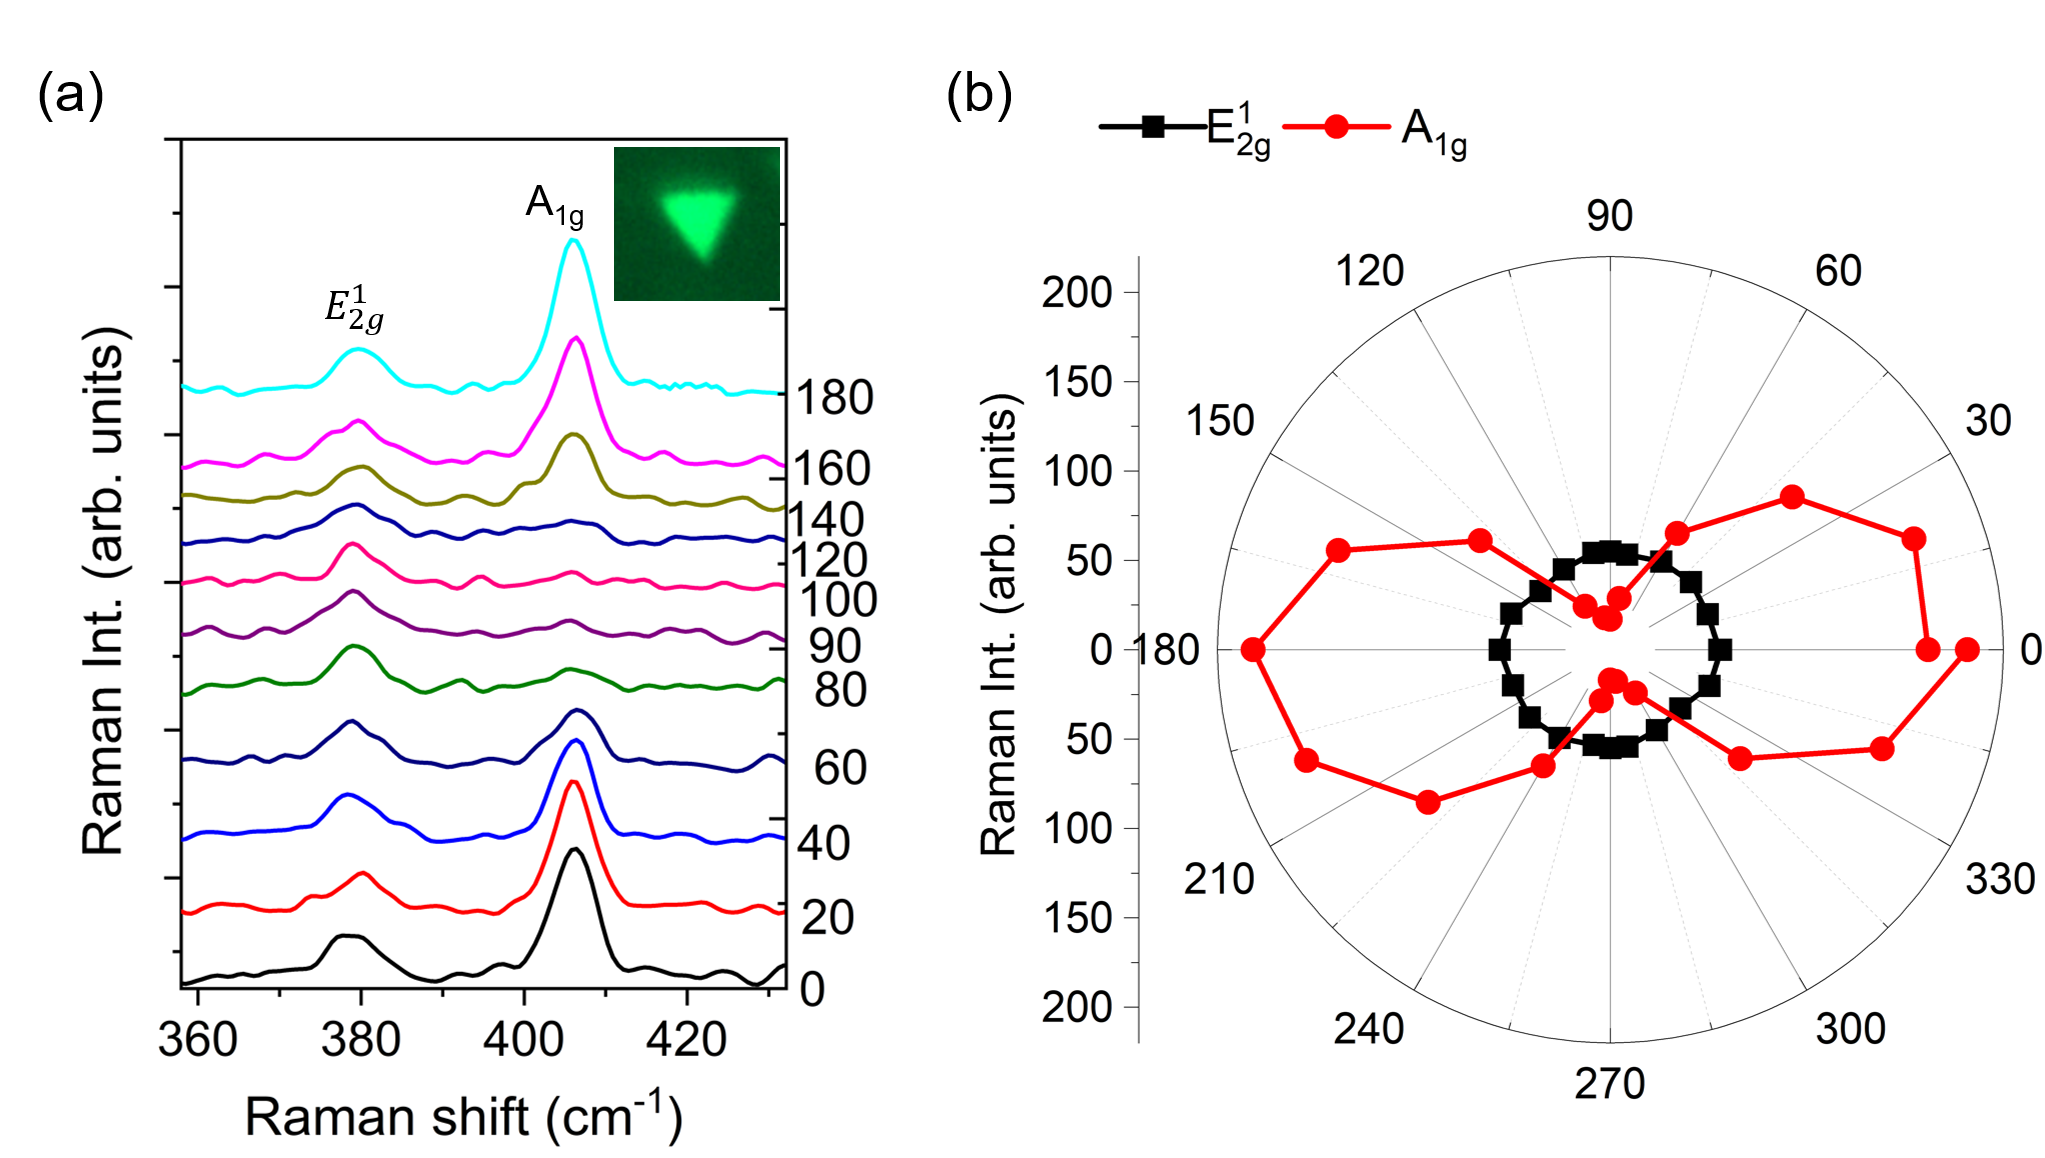
\includegraphics[width=0.9\linewidth]{Figures SI/Figure S3_polRaman triangle.png}
    \caption{\textbf{Polarization-resolved Raman measurements of monolayer triangular MoS$_2$.}. (a) Angle-dependent Raman spectra collected while rotating the monolayer sample from $0^{\circ}$ to $180^{\circ}$. 
    (b) Polar plots of the Raman intensity for the $E^1_{2g}$ (black) and $A_{1g}$ (red) phonon modes. The $E^1_{2g}$ mode exhibits an isotropic response, whereas the $A_{1g}$ mode shows pronounced twofold anisotropy, characteristic of 2H-phase monolayer MoS$_2$.} 
    \label{fig:si_2D_Triangular MoS2}
\end{figure}
\newpage
\section{Supplementary Note 4: Polarization-resolved Raman mapping of MoS$_2$ nanoribbons and comparison with triangular MoS$_2$}
\end{figure}

\begin{figure}%[htb]
    \centering 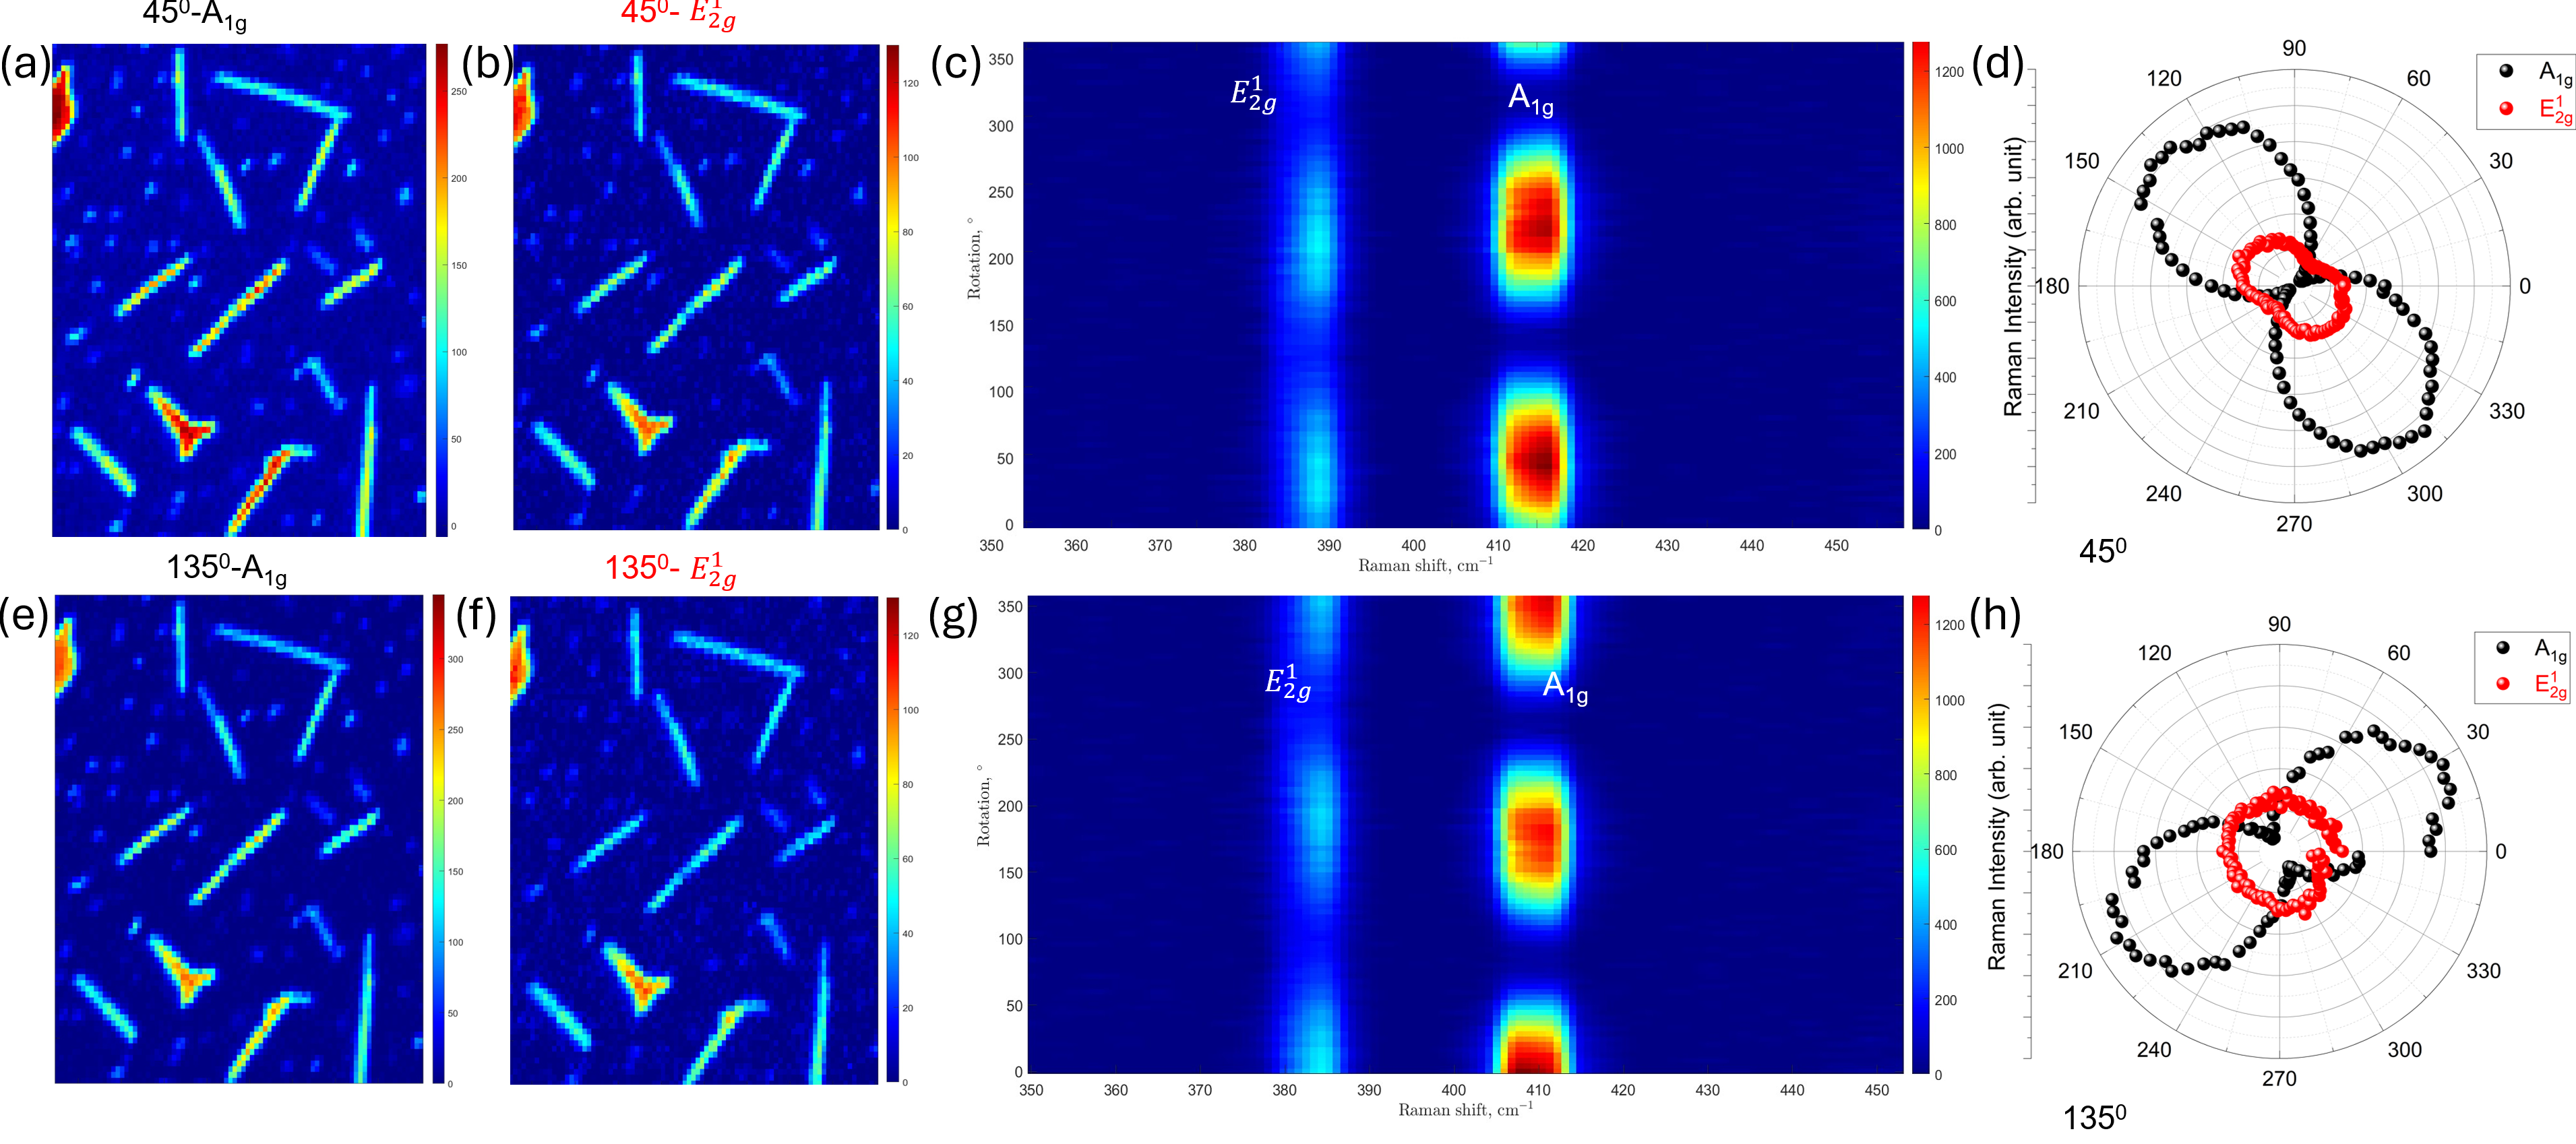
\includegraphics[width=1.0\linewidth]{Figures SI/Figure_S4_Polarization-resolved Raman mapping.png}
    \caption{\textbf{Polarization-resolved Raman mapping of MoS$_2$ nanoribbons.}.
(a,b) Raman intensity maps of the A$_{1g}$ and E$^1_{2g}$ modes acquired under an incident
polarization of $45^\circ$, with strong spatial contrast across individual nanoribbons.
(c) Angle-resolved Raman contour maps showing the evolution of the E$^1_{2g}$ and A$_{1g}$ (d) Corresponding polar plots of the Raman intensities for the A$_{1g}$ and E$^1_{2g}$ modes 
extracted from the $45^\circ$ rotational scans
(e,f) Raman maps measured under an incident polarization of $135^\circ$. 
(g) Angle-resolved Raman contour maps showing the evolution of the E$^1_{2g}$ and A$_{1g}$ at $135^\circ$ (h) Corresponding polar plots of the Raman intensities for the A$_{1g}$ and E$^1_{2g}$ modes 
extracted from the rotational scans.
}
\label{Fig_SI_4}
\end{figure}

Figure~S\ref {Fig_SI_4}a presents the polarization-dependent Raman response of MoS$_2$ nanoribbons, measured under cross-polarized excitation and detection geometries at $45^\circ$ and $135^\circ$. Panels (a,b,e,f) show spatial Raman maps of the A$_{1g}$ and E$^{1}_{2g}$ modes, revealing pronounced intensity variations as a function of both crystallographic orientation and polarization. The nanoribbons exhibit strong polarization contrast, where the Raman intensity of the out-of-plane A$_{1g}$ mode and the in-plane E$^{1}_{2g}$ mode both change significantly between the $45^\circ$ and $135^\circ$ configurations. 
Such behavior reflects the intrinsic structural anisotropy of quasi–one-dimensional MoS$_2$ nanoribbons. Their reduced lateral width induces symmetry breaking, modified Raman tensor elements, and strain gradients along the ribbon axis, all of which enhance polarization selectivity. The corresponding angle-resolved Raman maps in Figure~S\,4c,g further show that the E$^{1}_{2g}$ mode exhibits an asymmetric and highly angle-dependent intensity profile, whereas the A$_{1g}$ mode displays even larger modulation amplitude with a pronounced two-lobed pattern. These observations confirm a substantial in-plane anisotropy arising from the quasi-1D geometry and possible 3R-like stacking distortions generated during liquid-phase assisted growth.

The polar plots in Figure~S\ref {Fig_SI_4} d,h quantify the angular dependence of both Raman-active modes. The degree of polarization, calculated as $(I_{\parallel}-I_{\perp})/(I_{\parallel}+I_{\perp})$, yields distinctly non-zero values for both A$_{1g}$ and E$^{1}_{2g}$ modes in nanoribbons, unambiguously demonstrating anisotropic vibrational response. The strong modulation of the A$_{1g}$ mode, in particular, is consistent with symmetry breaking and non-uniform interlayer coupling within narrow MoS$_2$ ribbons.
For comparison, similar measurements performed on large-area monolayer triangular MoS$_2$ flakes display negligible angular dependence for the in-plane E$^{1}_{2g}$ mode and only weak modulation for the A$_{1g}$ mode. This isotropic behavior is expected for monolayer MoS$_2$ in the 2H phase, where the hexagonal symmetry enforces polarization-independent Raman response.
The clear contrast between the highly anisotropic nanoribbons and the nearly isotropic triangular domains highlights the role of reduced dimensionality in governing polarized Raman scattering. In 1D nanoribbons, strain, edge termination, and local symmetry breaking modify the Raman tensor elements, giving rise to the strong anisotropy observed in both modes. In contrast, 2H-phase triangular monolayers retain full in-plane symmetry and therefore show minimal polarization sensitivity. These results demonstrate that polarized Raman spectroscopy serves as a powerful diagnostic tool to distinguish between quasi-1D anisotropic MoS$_2$ nanostructures and their isotropic 2D counterparts.

\section {Supplementary Note 5: Width-Dependent Excitonic Anisotropy in MoS$_2$ Nanoribbons}

To further support the conclusions drawn in Figure.~4 of the main text, we performed
polarization-resolved differential reflectance measurements on an additional MoS$_2$
nanoribbon with a thickness of $\sim 30.2$~nm but a significantly larger width of
$\sim 600$~nm Figure~S\ref{fig:si_5_width_dependent_anisotropy}\,a. Despite its comparable thickness to the 
ribbon studied in Fig.~4 ($\sim 29.1$~nm) in the main text, the wider geometry produces a markedly 
different optical response. In particular, the excitonic resonances (Peaks~1 and~2) 
display almost isotropic polarization dependence, and the third low-energy feature 
exhibits only a weak signature of the Fabry--Pérot (FP) cavity mode. This stands in
contrast to the narrower $\sim 400$~nm ribbon in Figure.~4, in the main text peaks 2 and 3 show 
clear twofold anisotropy and the FP mode is strongly enhanced.
These observations indicate that lateral optical confinement plays a decisive role in establishing anisotropic exciton--photon coupling in quasi-1D MoS$_2$ nanoribbons. When the width increases, the effective in-plane cavity length becomes too large to 
support strong FP coupling, leading to suppressed anisotropy and spectral redshifting of the FP resonance. Conversely, narrower ribbons confine the optical field more efficiently, enabling pronounced angular modulation of both excitonic and FP-coupled 
features. This width dependence complements the main-text discussion and further confirms that the emergence of strong excitonic anisotropy in MoS$_2$ nanoribbons is a combined consequence of reduced dimensionality, modified stacking, and lateral photon confinement.
\begin{figure}%[htb]
    \centering
    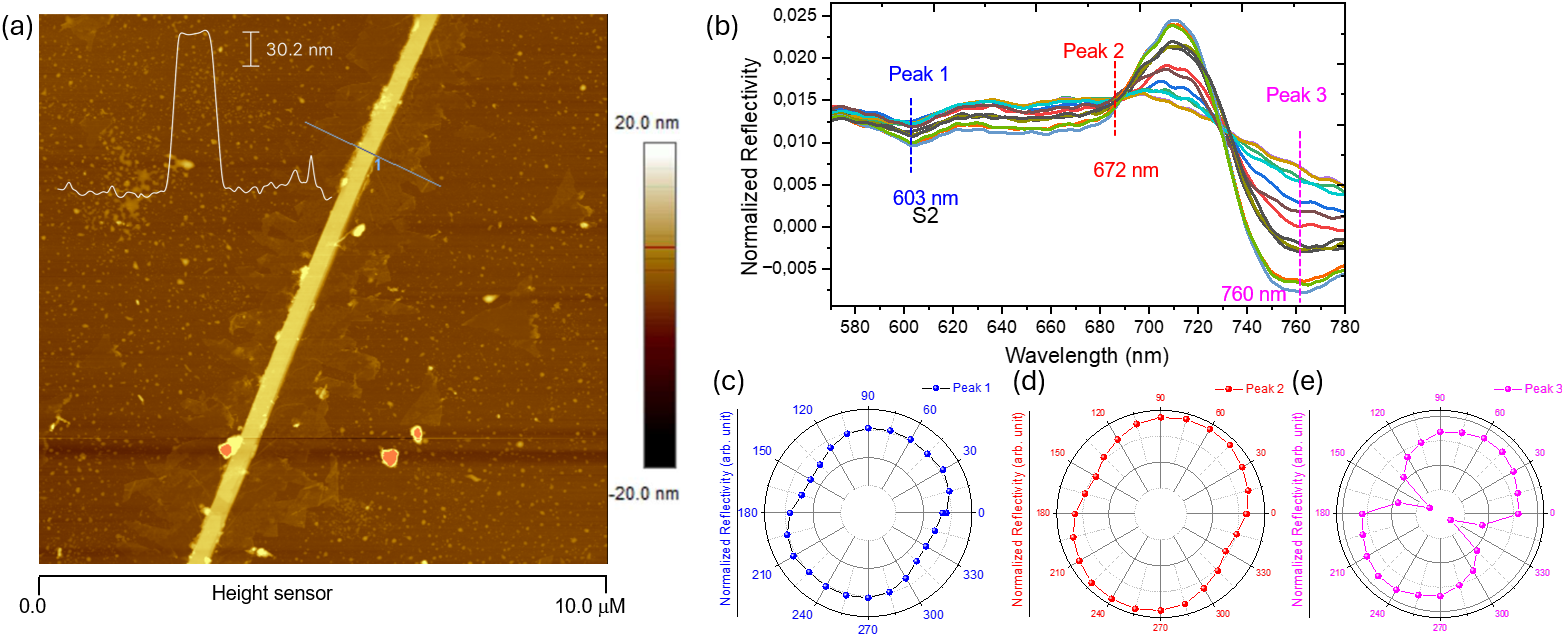
\includegraphics[width=1.0\linewidth]{Figures SI/Figure_S5_Width Dependent Excitonic Anisotrop.png}
\caption{\textbf{Polarization-resolved differential reflectance of a MoS$_2$ nanoribbon.}.
(a) AFM image of the nanoribbon showing a thickness of $\sim$30.2\,nm. 
(b) Normalized differential reflectance spectra measured as a function of incident polarization angle, revealing three optical resonances (Peak~1, Peak~2, and Peak~3). 
(c--e) Polar plots of the angular dependence of the three resonances. 
The broader nanoribbon exhibits modest anisotropy in Peak~1 and Peak~2, while Peak~3 (Fabry--Pérot-assisted mode) shows a stronger twofold modulation, reflecting the combined influence of ribbon geometry, thickness, and light matter coupling.} 
    \label{fig:si_5_width_dependent_anisotropy}
\end{figure}
\begin{figure}%[htb]
    \centering 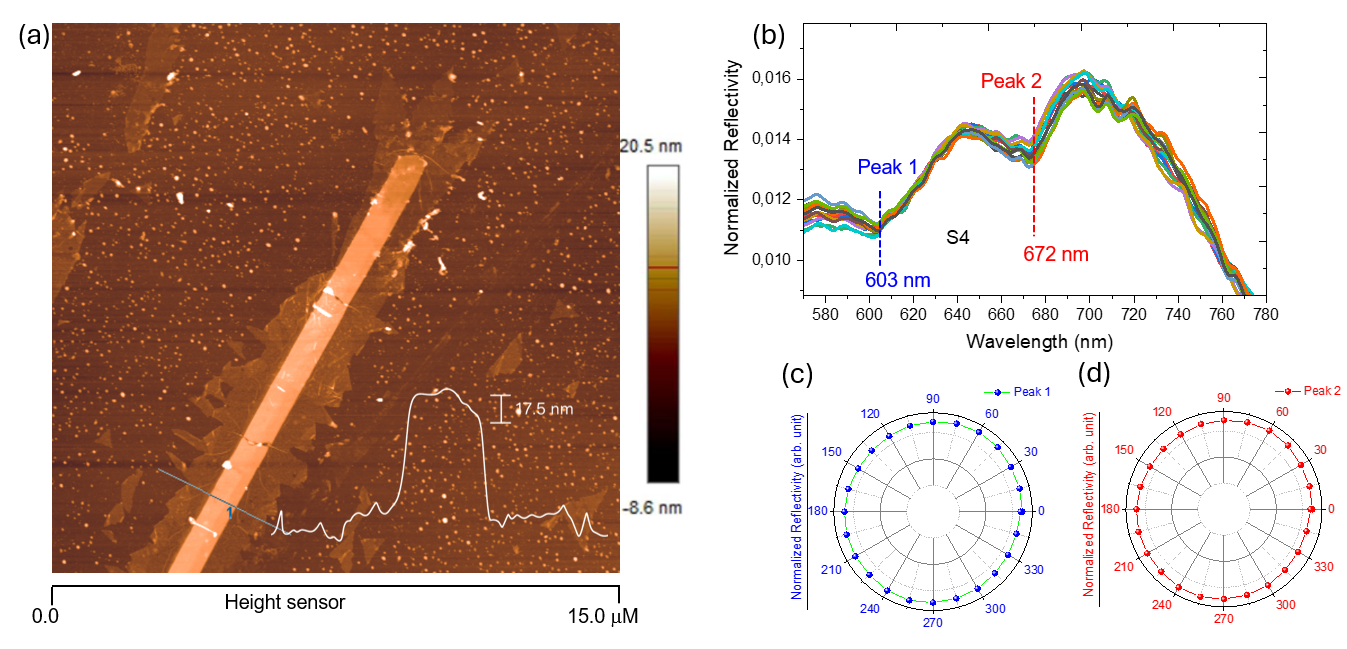
\includegraphics[width=1.0\linewidth]{Figures SI/Figure_S6_Width Dependent Excitonic Anisotropy.png}
    \caption{\textbf{Polarization-resolved differential reflectance of a MoS$_2$ nanoribbon}. (a) AFM image of the nanoribbon, showing a thickness of $\sim$17.5\,nm and a lateral width of $\sim$1\,$\mu$m.  (b) Polarization-dependent differential reflectance spectra measured while rotating the incident polarization from $0^{\circ}$ to $360^{\circ}$. In this relatively wide ribbon, only two optical resonances are observed at 603\,nm and 672\,nm (peak\,1 and peak\,2), while the Fabry--Pérot assisted mode that appears in narrower ribbons is absent.  (c, d) Polar plots of the angular dependence of peak\,1 and peak\,2 respectively. } \label{fig:si_6_width_dependent_anisotropy_wider}
\end{figure}

To further clarify the role of geometric confinement on the optical response, we investigated a MoS$_2$ nanoribbon with a relatively large width of $\sim 1~\mu$m and a smaller thickness of $\sim 17.5$ nm Figure~S\ref{fig:si_6_width_dependent_anisotropy_wider}. In contrast to the narrower and thicker nanoribbons discussed previously, this structure exhibits only two excitonic resonances at 603 nm and 672 nm (Peaks 1 and 2), while the Fabry–Pérot (FP) cavity mode observed in confined ribbons is absent. The absence of the FP resonance can be attributed to the combined effects of reduced vertical optical thickness and weak lateral confinement. Formation of FP-assisted modes requires sufficient cavity thickness to support standing optical waves together with lateral confinement that enhances photon localization along the ribbon axis. In the present ribbon, the small thickness ($\sim$17.5 nm) limits the effective optical cavity length, while the large lateral width suppresses in-plane confinement. As a result, the optical field cannot form a stable cavity resonance, and the spectrum is dominated solely by the intrinsic excitonic transitions. These results further confirm that the emergence of the FP-assisted resonance in MoS$_2$ nanoribbons requires a cooperative interplay between ribbon thickness and lateral confinement. Only when both conditions are satisfied, as in the narrower nanoribbons discussed in the main text, does strong cavity–exciton coupling appear, leading to the additional anisotropic resonance.

To further elucidate the role of lateral confinement on the optical anisotropy of 
quasi-1D MoS$_2$ nanoribbons, we performed polarization-dependent differential 
reflectance spectroscopy on a narrower ribbon with a thickness of 
$\sim 22.5$ nm and a lateral width of $\sim 300$ nm Figure~S\ref{fig:si_5_width_dependent_anisotropy_narrower}. 
In contrast to the wider ribbons presented in the main text, this highly confined 
structure exhibits \emph{three} well-defined resonant features at 
603 nm, 652 nm, and 681 nm (Peaks 1–3), all of which display strong and systematic 
angular modulation.

The emergence of the third resonance (Peak 3) and its clear twofold anisotropy 
indicate the formation of an enhanced Fabry–Pérot (FP) cavity along the confined ribbon axis. 
As the ribbon width decreases, the lateral optical path length becomes comparable to 
half-wavelength multiples of the excitonic transition energies. This condition favors the 
formation of guided FP cavity modes whose phase-matching couples efficiently with the intrinsic excitonic resonances. Consequently, FP modes become more pronounced and shift 
towards shorter wavelengths (higher energies), appearing closer to the intrinsic B exciton. 
Such behavior is expected for dielectric nanoresonators with reduced lateral dimensions, 
where modified boundary conditions compress the optical field and shift cavity resonances.
In addition, Peak 2 (the B exciton) exhibits a noticeable blue-shift relative to wider 
nanoribbons. This shift arises from enhanced lateral confinement, which modifies the 
effective dielectric screening and strengthens Coulomb interactions, thereby increasing 
the exciton binding energy. The resulting renormalization drives the B exciton to higher 
energy, consistent with the trend expected when transitioning from a quasi-2D layer to an 
increasingly anisotropic quasi-1D geometry. Polar plots of the three resonances Figure~S\ref{fig:si_5_width_dependent_anisotropy_narrower} c–e reveal pronounced twofold symmetry 
for all modes, significantly stronger than that observed in wider nanoribbons. This 
confirms that the narrowing of the ribbon enhances the directional dependence of light–
matter coupling by restricting exciton transport and optical field distribution along a 
single dominant axis. These findings provide compelling evidence that the optical 
Anisotropy in MoS$_2$ nanoribbons is highly tunable through geometric confinement, and 
that new FP-assisted resonances naturally emerge as the system approaches the 
quasi-1D limit.
\begin{figure}%[htb]
    \centering 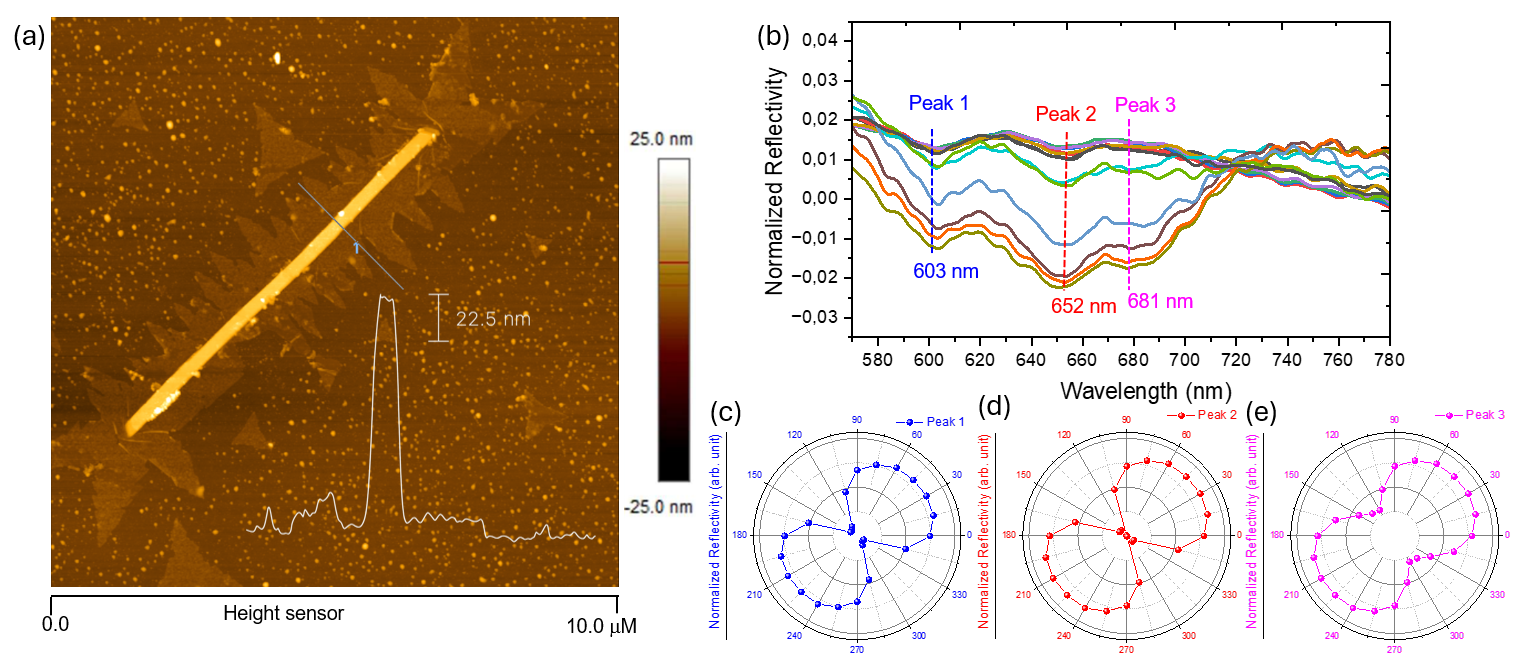
\includegraphics[width=1.0\linewidth]{Figures SI/Figure_S7_Width Dependent Excitonic Anisotropy.png}
    \caption{\textbf{Polarization-resolved differential reflectance of a narrow MoS$_2$ nanoribbon}. (a) AFM image of a nanoribbon with a thickness of $\sim22.5$ nm and a width of $\sim300$ nm. (b) Differential reflectance spectra measured as a function of incident polarization, showing three clear resonances at 603 nm, 652 nm, and 681 nm. (c–e) Polar plots of the angular dependence of the three resonances. The reduced ribbon width leads to pronounced anisotropy in all modes and the emergence of a strongly polarization-sensitive Fabry–Pérot (FP) resonance that shifts toward the excitonic energies due to enhanced lateral confinement and stronger cavity–exciton coupling.} 
\label{fig:si_5_width_dependent_anisotropy_narrower}
\end{figure}
\newpage
\end{document}


\bibliography{bibliography}




%%%%%%%%%%%%%%%%%%%%%%%%%%%%%%%%%%%%%%%%%%%%%%%%%%%%%%%%%%%%%%%%%%%%%%%%%%%%%%%%


